\documentclass{article}

\usepackage{graphicx}
\usepackage[margin=2cm]{geometry}
\usepackage{verbatim}
\usepackage[export]{adjustbox}

\begin{document}

\newcommand{\modefont}[1]{\texttt{#1}}
\newcommand{\mnocheck}{\modefont{nocheck}}
\newcommand{\mnonstrict}{\modefont{nonstrict}}
\newcommand{\mstrict}{\modefont{strict}}

%% ---
\subsection*{Figure 3: Records per Hour}

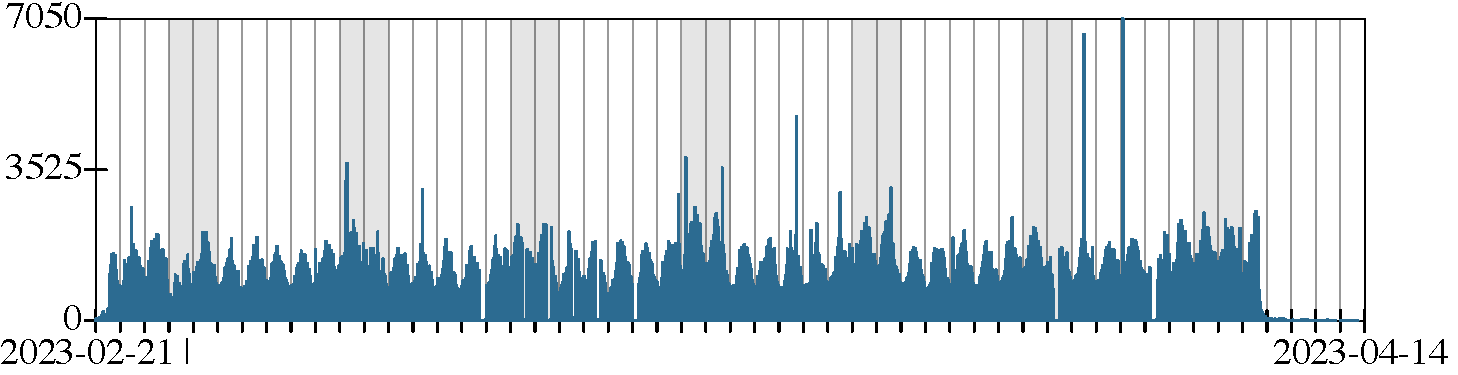
\includegraphics[width=\columnwidth]{out/row-distribution.pdf}

Lines 1-2 of \texttt{out/overview.txt} give the reason for sending:

\begin{verbatim}
 1504736 total logs = 1341348 nocheck + 156883 nonstrict + 6505 strict
  508572 due to module switch
\end{verbatim}


%% ---
\subsection*{Table 2: Size of Analyzed Code}

From \texttt{out/summary-of-size-distributions.rktd}:

{\footnotesize
\verbatiminput{out/summary-of-size-distributions.rktd}
}

\begin{minipage}{0.5\columnwidth}
  \textbf{Lines:}\\
  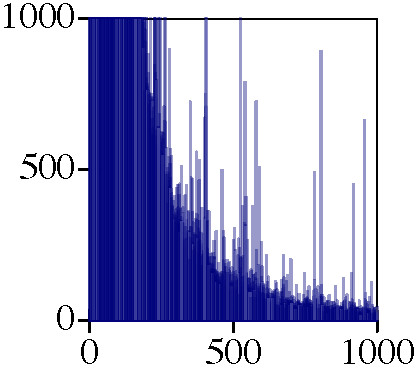
\includegraphics[width=\columnwidth]{out/lines-distribution.pdf}
\end{minipage}\begin{minipage}{0.5\columnwidth}
  \textbf{Edit Range:}\\
  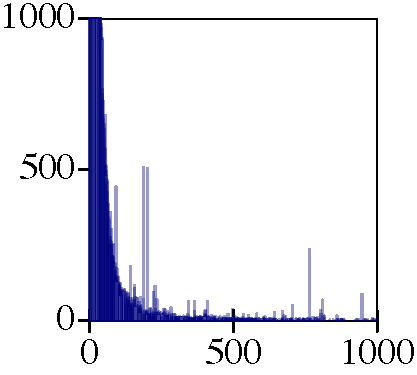
\includegraphics[width=\columnwidth]{out/editrange-distribution.pdf}
\end{minipage}


%% ---
\subsection*{Table 3: Session Size}

See previous section for mean, stddev, median, and P99.

\begin{minipage}{0.5\columnwidth}
  \textbf{Timespan:}
  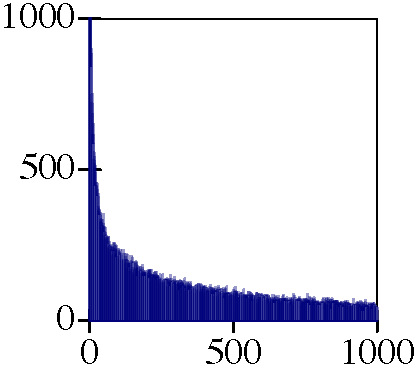
\includegraphics[width=0.4\columnwidth]{out/timespan-distribution.pdf}
\end{minipage}\begin{minipage}{0.5\columnwidth}
  \textbf{Event Count / Record Count:}
  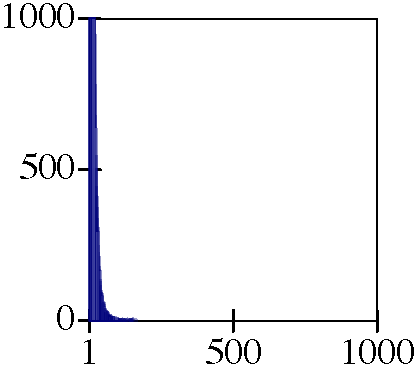
\includegraphics[width=0.4\columnwidth]{out/event-count-distribution.pdf}
\end{minipage}


%% ---
\subsection*{Table 4: Current Type Errors and Background Errors}

Lines 3-8 of \texttt{out/overview.txt}:

\begin{verbatim}
 72235735 total forced strict type errors, 37027281 in module,
 curr 1111178 in edit regions,
 olde 938500 in edit regions
 595137 total type errors, 289698 in module,
 curr 14917 non-stx + 16007 syntax in edit regions,
 olde 13836 non-stx + 28565 syntax in edit regions
\end{verbatim}


%% ---
\subsection*{Figure 4: Overview of Type Analysis Modes}

Line 1 of \texttt{out/overview.txt} partitions logs by mode:

\begin{verbatim}
 1504736 total logs = 1341348 nocheck + 156883 nonstrict + 6505 strict
\end{verbatim}

Lines 9-13 of \texttt{out/overview.txt} partition sessions and report on upgrades and downgrades,
\emph{but} the final two numbers are incorrect (upgrade and downgrade) because they include
module switches:

\begin{verbatim}
 347598 sessions
  346956 single mode = 313509 nocheck + 32902 nonstrict + 545 strict
  512 multi mode projects
  341 mode upgrades
  320 mode downgrades
\end{verbatim}

Correct up/down-grade numbers are in \texttt{out/downgrade-count.txt}:

\includeverbatim{out/downgrade-count.txt}

TODO ^^^


%% ---
\subsection*{Figure 5: Type and Background Errors Grouped by Mode}

{ \newcommand{\labelbars}[1]{\begin{tabular}[t]{l@{}l} \raisebox{2ex}{\begin{tabular}[t]{r}\mnocheck{}\\\mnonstrict{}\\\mstrict{}\end{tabular}} & #1 \end{tabular}}
  \begin{tabular}[t]{cc}
    Type errors & Background errors \\
    \labelbars{\includegraphics[width=0.20\columnwidth,valign=M]{out/error-by-mode-te.pdf}}
    & \labelbars{\includegraphics[width=0.20\columnwidth,valign=M]{out/error-by-mode-fs.pdf}}
  \end{tabular}
}


%% ---
\subsection*{Table 5: Specific Errors in Edit Range}

TODO


%% ---
\subsection*{Table 6: Type Error Popularity}

TODO

{\footnotesize
\verbatiminput{out/ctc-info.txt}
}


%% ---
\subsection*{Figure 6: Type Error Density}

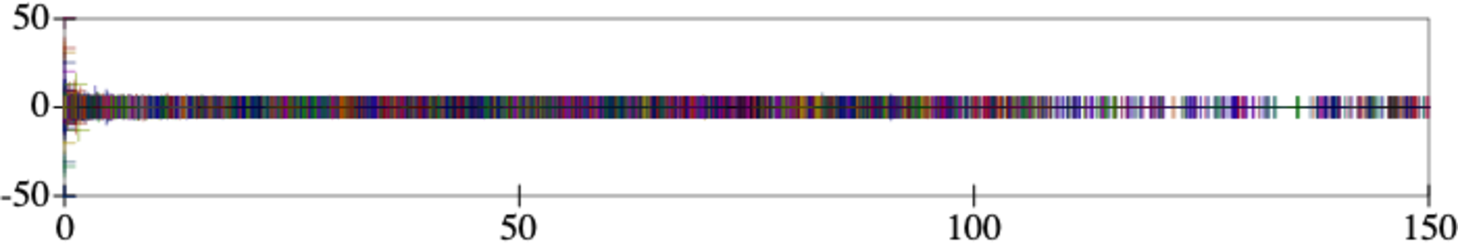
\includegraphics[width=\columnwidth]{out/error-count-nocheck-row--te-density-diff.pdf}
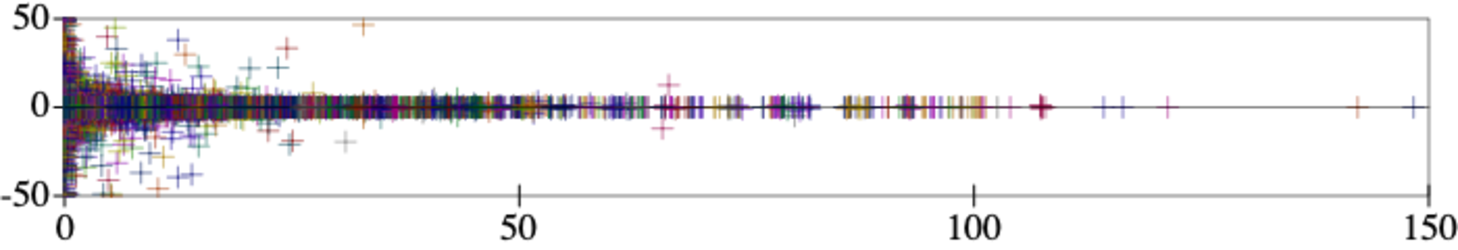
\includegraphics[width=\columnwidth]{out/error-count-nonstrict-row--te-density-diff.pdf}
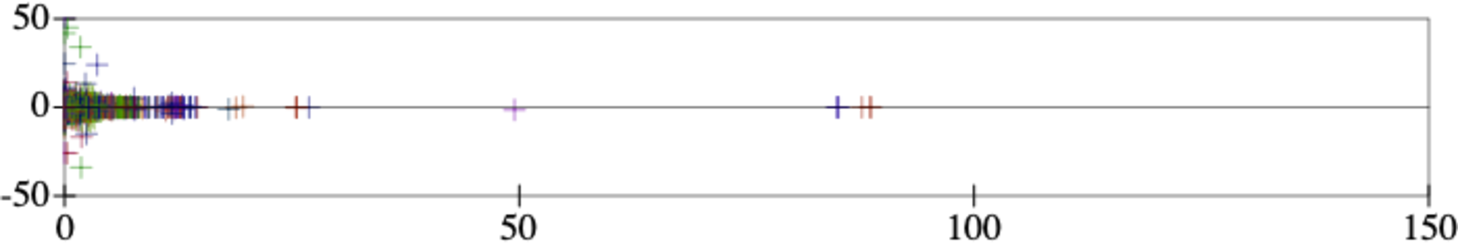
\includegraphics[width=\columnwidth]{out/error-count-strict-row--te-density-diff.pdf}


\end{document}
